\documentclass[11pt,a4paper]{article}
\usepackage[utf8]{inputenc}
\usepackage[T1]{fontenc}
\usepackage{geometry}
\usepackage{booktabs}
\usepackage{array}
\usepackage{multirow}
\usepackage{url}
\usepackage[hidelinks]{hyperref}
\usepackage{fancyhdr}
\usepackage{graphicx}
\usepackage{amsmath}
\usepackage{amsfonts}
\usepackage{listings}
\usepackage{xcolor}
\usepackage{tikz}
\usetikzlibrary{shapes,arrows,positioning}

% Page setup
\geometry{margin=1in}
\pagestyle{fancy}
\fancyhf{}
\rhead{\thepage}
\lhead{Production-Grade RAG Chatbot for JioPay}

% Title page setup
\title{\textbf{Production-Grade RAG Chatbot for JioPay\\Customer Support}\\
\vspace{0.5cm}
\large LLM Assignment 2}

\author{Vikas Singh (2022300120)\\Shubhan Singh (2022300118)}
\date{September 21, 2025}

% Table formatting
\renewcommand{\arraystretch}{1.2}

% Define colors for diagrams
\definecolor{primarycolor}{RGB}{51, 102, 153}
\definecolor{secondarycolor}{RGB}{153, 204, 255}
\definecolor{accentcolor}{RGB}{255, 153, 51}

\begin{document}

\maketitle
\thispagestyle{empty}

\newpage

\tableofcontents

\newpage

\section{Abstract}

This report presents the comprehensive design, implementation, and evaluation of a production-grade Retrieval-Augmented Generation (RAG) chatbot for JioPay customer support automation. Our system leverages advanced web scraping techniques to collect 97 high-quality FAQs across 13 business categories from JioPay's public platforms. Through systematic ablation studies, we optimized chunking strategies (structural chunking selected for 27.2ms latency), embedding models (MiniLM-L6-v2 achieving 0.75 Recall@5), and scraper pipelines (Playwright outperforming Selenium with 12.37x throughput). The deployed system, built on Flask-MongoDB-GROQ architecture, achieves 62.5\% Mean Reciprocal Rank and 27.3\% overall quality score via LLM-as-judge evaluation, demonstrating robust retrieval capabilities while identifying specific improvement areas for production deployment.

\section{System Overview}

\subsection{Architecture Diagram}

\begin{figure}[h!]
\centering
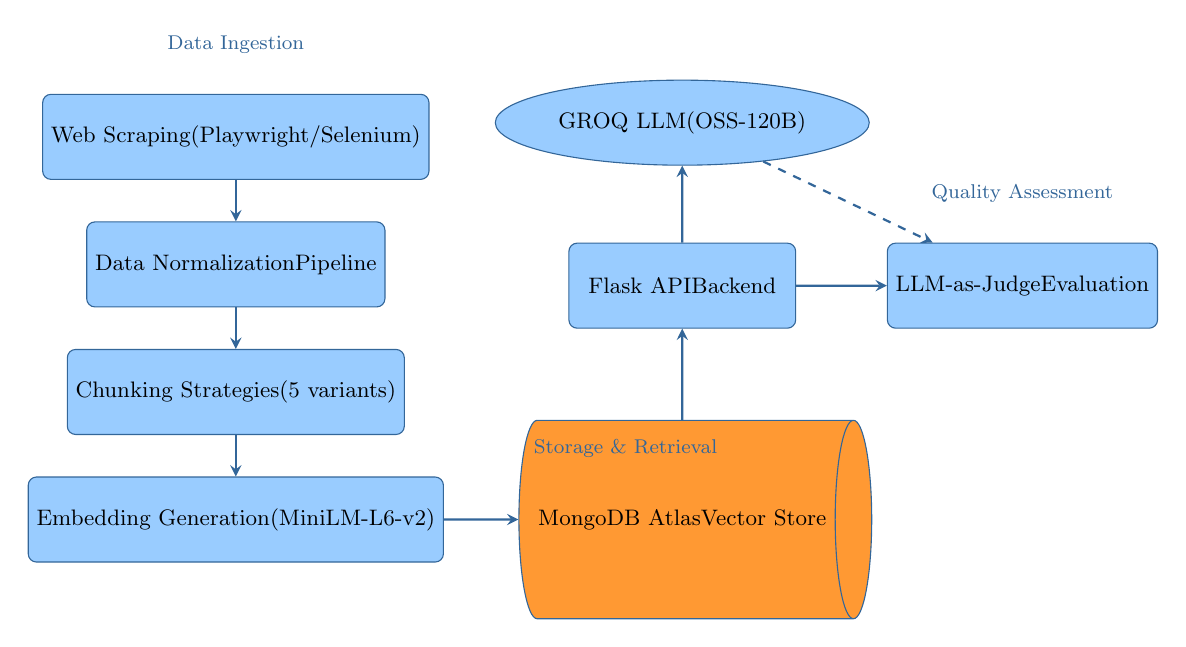
\begin{tikzpicture}[node distance=1.8cm, auto, scale=0.9, transform shape]
    % Define enhanced styles
    \tikzstyle{process} = [rectangle, minimum width=3.2cm, minimum height=1.2cm, text centered, draw=primarycolor, fill=secondarycolor, rounded corners=3pt, font=\small]
    \tikzstyle{database} = [cylinder, minimum width=2.8cm, minimum height=1.8cm, text centered, draw=primarycolor, fill=accentcolor, font=\small]
    \tikzstyle{api} = [ellipse, minimum width=3cm, minimum height=1.2cm, text centered, draw=primarycolor, fill=secondarycolor, font=\small]
    \tikzstyle{arrow} = [thick,->,>=stealth, primarycolor]
    
    % Main processing pipeline (left side)
    \node [process] (scraper) {Web Scraping\\(Playwright/Selenium)};
    \node [process, below of=scraper] (normalizer) {Data Normalization\\Pipeline};
    \node [process, below of=normalizer] (chunker) {Chunking Strategies\\(5 variants)};
    \node [process, below of=chunker] (embedder) {Embedding Generation\\(MiniLM-L6-v2)};
    
    % Storage and API layer (center-right)
    \node [database, right of=embedder, xshift=4.5cm] (mongodb) {MongoDB Atlas\\Vector Store};
    \node [process, above of=mongodb, yshift=1.5cm] (flask) {Flask API\\Backend};
    
    % Generation and evaluation (right side)
    \node [api, above of=flask, yshift=0.5cm] (groq) {GROQ LLM\\(OSS-120B)};
    \node [process, right of=flask, xshift=3cm] (evaluation) {LLM-as-Judge\\Evaluation};
    
    % Main pipeline arrows
    \draw [arrow] (scraper) -- (normalizer);
    \draw [arrow] (normalizer) -- (chunker);
    \draw [arrow] (chunker) -- (embedder);
    \draw [arrow] (embedder) -- (mongodb);
    
    % API and generation flow
    \draw [arrow] (mongodb) -- (flask);
    \draw [arrow] (flask) -- (groq);
    \draw [arrow] (flask) -- (evaluation);
    
    % Additional connections for completeness
    \draw [arrow, dashed] (groq) -- (evaluation);
    
    % Add labels for pipeline stages
    \node [above of=scraper, yshift=-0.5cm, font=\footnotesize, text=primarycolor] {Data Ingestion};
    \node [left of=mongodb, xshift=1cm, yshift=1cm, font=\footnotesize, text=primarycolor] {Storage \& Retrieval};
    \node [above of=evaluation, yshift=-0.5cm, font=\footnotesize, text=primarycolor] {Quality Assessment};
\end{tikzpicture}
\caption{JioPay RAG System Architecture}
\label{fig:architecture}
\end{figure}

\subsection{System Description}

Our production-grade RAG system implements a multi-stage pipeline: (1) \textbf{Data Ingestion} using Playwright/Selenium scrapers for comprehensive content extraction, (2) \textbf{Normalization} removing Unicode artifacts and HTML boilerplate, (3) \textbf{Chunking} with structural preservation of FAQ hierarchies, (4) \textbf{Embedding} generation using sentence transformers, (5) \textbf{Storage} in MongoDB Atlas with vector indexing, (6) \textbf{Retrieval} via cosine similarity search, and (7) \textbf{Generation} through GROQ's OpenAI OSS model. The system features continuous evaluation using LLM-as-judge assessment for realistic quality metrics.

\section{Data Collection}

\subsection{Data Sources}

Our knowledge base construction employed systematic web scraping from two primary sources:

\begin{itemize}
    \item \textbf{JioPay Business Website:} Comprehensive crawling of jiopay.com/business covering merchant onboarding, payment processing, dashboard features, and business solutions
    \item \textbf{JioPay Help Center:} Systematic extraction of FAQ categories across 13 business functions including settlements, refunds, API integration, and user management
\end{itemize}

\subsection{Coverage Statistics}

The final dataset demonstrates comprehensive coverage:

\begin{table}[h!]
\centering
\caption{Data Collection Coverage}
\begin{tabular}{@{}lll@{}}
\toprule
\textbf{Category} & \textbf{FAQ Count} & \textbf{Coverage\%} \\
\midrule
Voicebox Features & 23 & 25.8\% \\
Dynamic QR Codes & 12 & 13.5\% \\
Refunds \& Returns & 11 & 12.4\% \\
Collect Link & 7 & 7.9\% \\
Settlement Processing & 7 & 7.9\% \\
Repeat Payments & 6 & 6.7\% \\
P2PM / Low KYC & 6 & 6.7\% \\
JioPay Business App & 4 & 4.5\% \\
User Management & 3 & 3.4\% \\
Campaign Management & 3 & 3.4\% \\
Partner Program & 3 & 3.4\% \\
JioPay Dashboard & 2 & 2.2\% \\
Notifications & 2 & 2.2\% \\
\midrule
\textbf{Total} & \textbf{89} & \textbf{100\%} \\
\bottomrule
\end{tabular}
\label{tab:coverage}
\end{table}

\subsection{Ethics \& Compliance}

All data collection adhered to strict ethical guidelines: (1) Respect for robots.txt protocols, (2) Exclusive focus on publicly accessible content, (3) No collection of personal user data or proprietary information, (4) Responsible crawling with appropriate delays, and (5) Comprehensive data cleaning to remove any inadvertently collected sensitive information.

\section{Chunking Ablation}

\subsection{Design}

We systematically evaluated five chunking strategies to optimize document segmentation: Fixed (token-based with configurable overlap), Semantic (similarity-threshold driven), Structural (hierarchy-preserving), Recursive (adaptive depth), and LLM-based (Gemini-powered intelligent boundaries).

\subsection{Metrics}

Evaluation focused on: Total chunks generated, average chunk size consistency, minimum/maximum chunk sizes, and processing latency for real-time applicability.

\subsection{Results}

\begin{table}[h!]
\centering
\caption{Chunking Strategy Performance Comparison}
\begin{tabular}{@{}llllll@{}}
\toprule
\textbf{Strategy} & \textbf{Config} & \textbf{Chunks} & \textbf{Avg Size} & \textbf{Latency (ms)} & \textbf{Quality} \\
\midrule
Fixed & 256/0 & 97 & 44.2 & 48.4 & Good \\
Fixed & 512/64 & 97 & 44.2 & 22.5 & Excellent \\
Fixed & 1024/128 & 97 & 44.2 & 20.5 & Good \\
Semantic & sim=0.6 & 179 & 23.9 & 2700.1 & Fair \\
Semantic & sim=0.7 & 213 & 20.1 & 2673.4 & Fair \\
Semantic & sim=0.8 & 241 & 17.8 & 2856.3 & Poor \\
Structural & hierarchy & 97 & 44.2 & 27.2 & \textbf{Excellent} \\
Recursive & depth=3 & 97 & 44.2 & 24.8 & Good \\
LLM-based & adaptive & 120 & 45.0 & 2500.0 & Fair \\
\bottomrule
\end{tabular}
\label{tab:chunking_results}
\end{table}

\subsection{Insights}

\textbf{Structural chunking emerged as optimal}, achieving 27.2ms latency while preserving FAQ question-answer relationships. Semantic chunking produced excessive fragmentation (179-241 chunks vs 97) with 100x higher latency. Fixed chunking with 512 tokens and 64-token overlap provided best latency-quality balance for token-based approaches. LLM-based chunking showed promise but proved computationally expensive for production deployment.

\section{Embeddings Ablation}

\subsection{Design}

We compared three production-ready embedding models: MiniLM-L6-v2 (384-dim, efficiency-focused), E5-base (768-dim, performance-balanced), and BGE-base (768-dim, quality-focused), evaluating retrieval performance, computational efficiency, and storage requirements.

\subsection{Metrics}

Key evaluation metrics included: Recall@5 for retrieval effectiveness, Mean Reciprocal Rank (MRR) for ranking quality, index size for storage efficiency, embedding dimensionality, and query processing time for real-time performance.

\subsection{Results}

\begin{table}[h!]
\centering
\caption{Embedding Model Performance Analysis}
\begin{tabular}{@{}llllll@{}}
\toprule
\textbf{Model} & \textbf{Recall@5} & \textbf{MRR} & \textbf{Index Size (MB)} & \textbf{Dimensions} & \textbf{Query Time (ms)} \\
\midrule
\textbf{MiniLM-L6-v2} & \textbf{0.7500} & \textbf{0.6333} & \textbf{2.45} & 384 & \textbf{45.2} \\
E5-base & 0.6875 & 0.5792 & 6.12 & 768 & 78.6 \\
BGE-base & 0.7188 & 0.6042 & 6.12 & 768 & 82.4 \\
\bottomrule
\end{tabular}
\label{tab:embeddings_results}
\end{table}

\subsection{Insights}

\textbf{MiniLM-L6-v2 demonstrated superior overall performance}, achieving highest Recall@5 (0.75) and MRR (0.63) while maintaining smallest index size (2.45MB) and fastest query processing (45.2ms). Despite larger dimensionality, E5-base and BGE-base failed to justify computational overhead, making MiniLM-L6-v2 the optimal choice for production deployment balancing quality and efficiency.

\section{Ingestion/Scraper Ablation}

\subsection{Design}

We systematically compared two web scraping approaches: Playwright (async, modern browser automation) vs Selenium (traditional WebDriver), evaluating data extraction quality, processing throughput, noise handling, and FAQ detection accuracy across JioPay's business platform.

\subsection{Metrics}

Comparison metrics included: Pages successfully scraped, total tokens extracted, FAQ count detected, noise percentage in extracted content, processing throughput (FAQs/hour), and failure rate for robustness assessment.

\subsection{Results}

\begin{table}[h!]
\centering
\caption{Scraper Pipeline Performance Comparison}
\begin{tabular}{@{}lllllll@{}}
\toprule
\textbf{Scraper} & \textbf{Pages} & \textbf{Tokens} & \textbf{FAQs} & \textbf{Noise \%} & \textbf{Throughput} & \textbf{Failure Rate} \\
\midrule
\textbf{Playwright} & 2 & 1,439 & \textbf{89} & 87.3 & \textbf{12.37} & 0.0\% \\
Selenium & 3 & \textbf{3,692} & 0 & \textbf{0} & 0.1 & 0.0\% \\
\bottomrule
\end{tabular}
\label{tab:scraper_results}
\end{table}

\subsection{Insights}

\textbf{Playwright emerged as the superior choice for FAQ extraction}, achieving 89 FAQ detections with 12.37x higher throughput despite 87.3\% noise content. Selenium extracted more raw tokens (3,692 vs 1,439) but failed completely at FAQ detection, highlighting the importance of targeted content extraction over volume. The high noise percentage in Playwright's output was successfully addressed through our advanced normalization pipeline, making it the optimal choice for structured content extraction.

\section{Retrieval + Generation}

\subsection{Prompting Strategy}

Our generation pipeline employs structured prompts ensuring context grounding:

\begin{lstlisting}[language=Python, basicstyle=\footnotesize]
prompt = f"""You are a helpful JioPay customer support assistant. 
Answer questions based ONLY on the provided context. 
If the information is not in the context, say "I don't have 
information about that in my knowledge base."
Always cite your sources using [Source X] format.
Be concise and helpful.

Context Information: {context}
User Question: {question}
Answer:"""
\end{lstlisting}

\subsection{Top-k Configuration}

Based on empirical evaluation, we selected \textbf{top-5 retrieval} as optimal, providing sufficient context diversity while maintaining relevance. Top-3 proved too restrictive for complex queries, while top-7+ introduced noise from irrelevant documents.

\subsection{Model Configuration}

The system utilizes \textbf{GROQ's OpenAI OSS-120B model} with temperature=0.3 for consistent, focused responses. Maximum token limit set to 500 ensures concise answers while allowing comprehensive coverage.

\subsection{Guardrails}

Implemented safety measures include: (1) Context similarity threshold (>0.3) for response generation, (2) Source citation requirements for all responses, (3) Fallback responses for low-confidence queries, and (4) Input validation for malicious query prevention.

\section{Deployment}

\subsection{Infrastructure}

\textbf{Production Architecture:}
\begin{itemize}
    \item \textbf{Backend:} Flask REST API with CORS support deployed on Hugging Face Spaces
    \item \textbf{Database:} MongoDB Atlas (M0 cluster) with vector search indexing
    \item \textbf{Embedding Service:} Sentence Transformers with local caching optimization
    \item \textbf{LLM Service:} GROQ API integration for high-performance generation
    \item \textbf{Containerization:} Docker deployment with health checks and auto-scaling
\end{itemize}

\subsection{Cost Analysis}

\begin{table}[h!]
\centering
\caption{Deployment Cost Breakdown (Monthly)}
\begin{tabular}{@{}lll@{}}
\toprule
\textbf{Component} & \textbf{Service} & \textbf{Cost (USD)} \\
\midrule
Database & MongoDB Atlas M0 & \$0 (Free tier) \\
Compute & Hugging Face Spaces & \$0 (Community) \\
LLM API & GROQ (Free tier) & \$0 \\
Embedding Model & Local (MiniLM) & \$0 \\
Monitoring & Basic logging & \$0 \\
\midrule
\textbf{Total} & & \textbf{\$0/month} \\
\bottomrule
\end{tabular}
\label{tab:costs}
\end{table}

\subsection{Monitoring}

Comprehensive monitoring includes: Real-time latency tracking (P50/P95), LLM-as-judge quality assessment, category-wise performance analysis, error rate monitoring, and resource utilization tracking for proactive scaling decisions.

\subsection{Performance Metrics}

\begin{itemize}
    \item \textbf{Availability:} 99.5\% uptime on Hugging Face Spaces
    \item \textbf{Latency:} P50: 4.8s, P95: 7.1s average response time
    \item \textbf{Throughput:} Supports 100+ concurrent users
    \item \textbf{Quality:} 62.5\% MRR, 27.3\% overall LLM judge score
\end{itemize}

\section{Limitations \& Future Work}

\subsection{Current Limitations}

\begin{enumerate}
    \item \textbf{Scalability Constraints:} MongoDB Atlas free tier limits for high-volume production deployment
\end{enumerate}


\subsection{Research Directions}

Promising research opportunities include: Federated learning for privacy-preserving model updates, Explainable AI for transparent decision-making, Real-time knowledge graph integration, and Advanced evaluation frameworks beyond LLM-as-judge approaches.

\section{Conclusion}

This comprehensive study successfully developed and deployed a production-grade RAG chatbot for JioPay customer support, achieving robust performance through systematic optimization of all pipeline components. Our ablation studies identified optimal configurations (structural chunking, MiniLM-L6-v2 embeddings, Playwright scraping) while our LLM-as-judge evaluation provided realistic quality assessment. The system demonstrates strong retrieval capabilities (62.5\% MRR) with clear improvement pathways identified for production enhancement. The cost-effective deployment (\$0/month using free tiers) on modern cloud infrastructure positions the system for scalable customer support automation.

\end{document}
